\section{General Attention Layer}
\begin{frame}{}
    \LARGE Advanced Computer Vision: \textbf{General Attention Layer}
\end{frame}

\begin{frame}{Attention We Just Saw in Image Captioning}
\begin{figure}
\centering
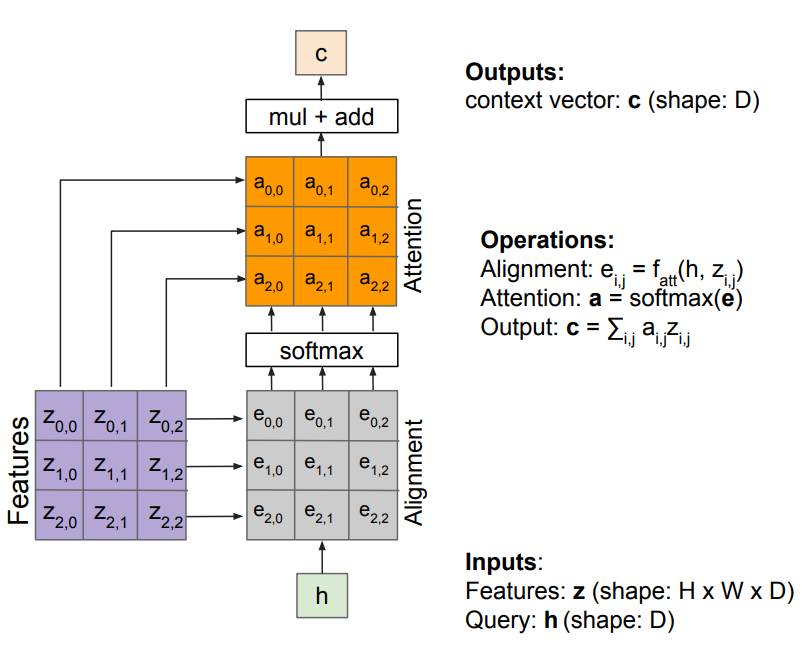
\includegraphics[width=1.0\textwidth,height=0.9\textheight,keepaspectratio]{images/advanced-cv/attention_20.png}
\end{figure} 
\end{frame}

\begin{frame}{General Attention Layer}
\begin{columns}
    
    \begin{column}{0.6\textwidth}
    \only<1>{
    \begin{figure}
    \centering
    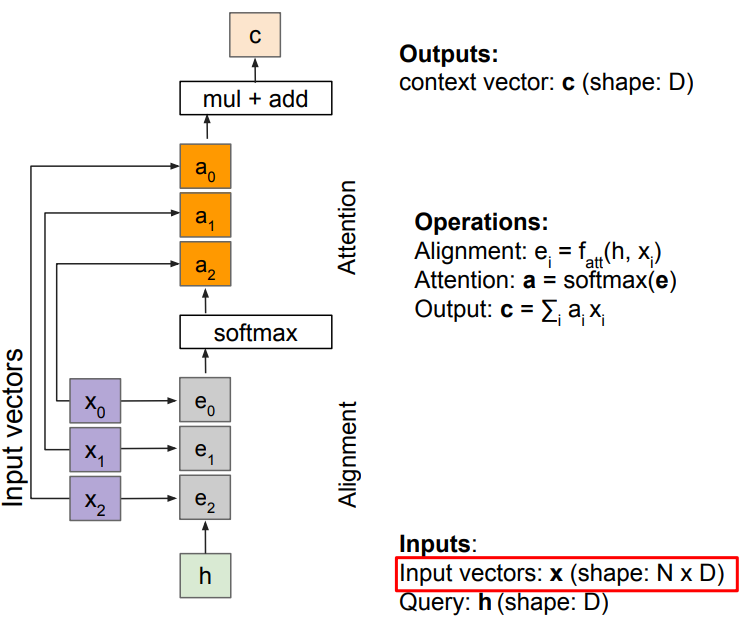
\includegraphics[width=1.0\textwidth,height=1.0\textheight,keepaspectratio]{images/advanced-cv/attention_21.png}
    \end{figure}
    }

    \only<2>{
    \begin{figure}
    \centering
    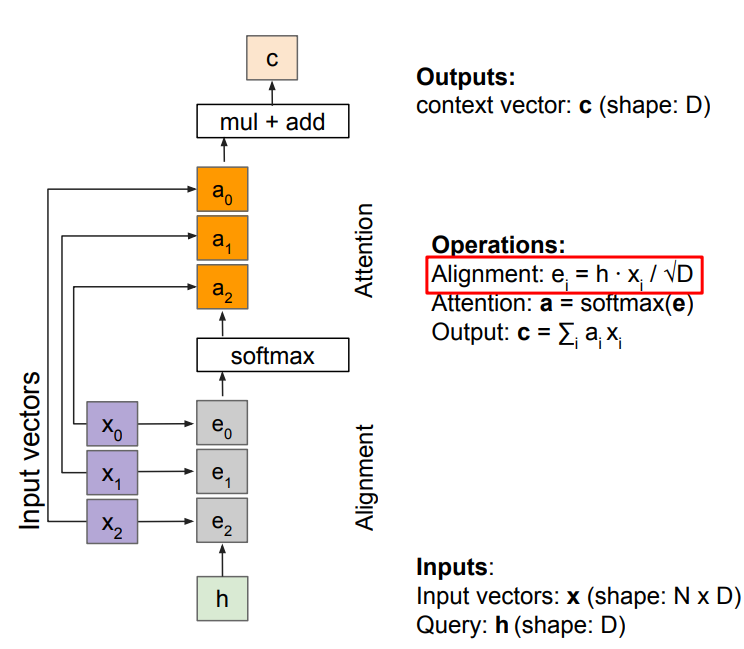
\includegraphics[width=1.0\textwidth,height=1.0\textheight,keepaspectratio]{images/advanced-cv/attention_22.png}
    \end{figure}
    }

    \only<3>{
    \begin{figure}
    \centering
    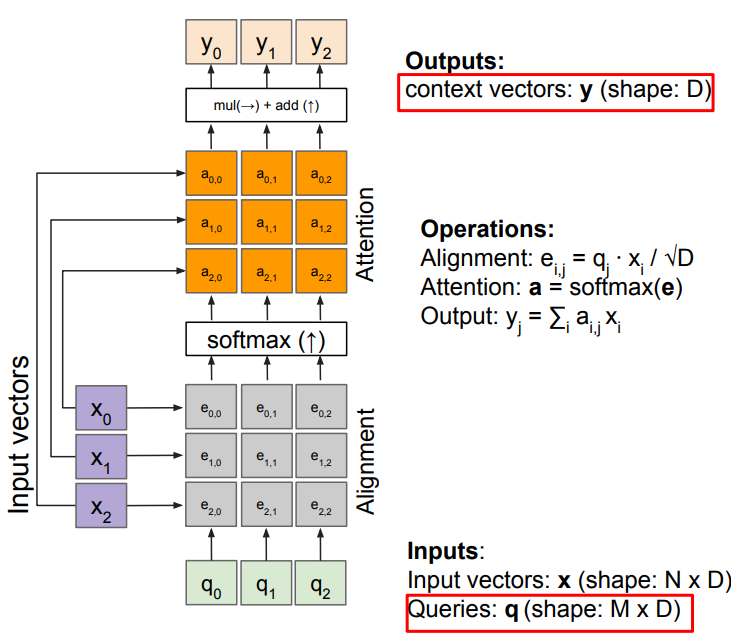
\includegraphics[width=1.0\textwidth,height=1.0\textheight,keepaspectratio]{images/advanced-cv/attention_23.png}
    \end{figure}
    }

    \only<4>{
    \begin{figure}
    \centering
    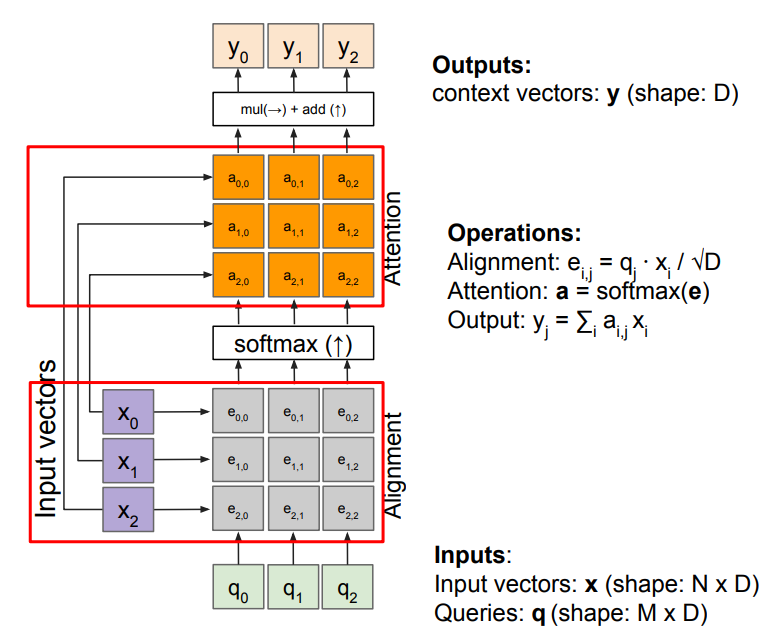
\includegraphics[width=1.0\textwidth,height=1.0\textheight,keepaspectratio]{images/advanced-cv/attention_24.png}
    \end{figure}
    }

    \only<5>{
    \begin{figure}
    \centering
    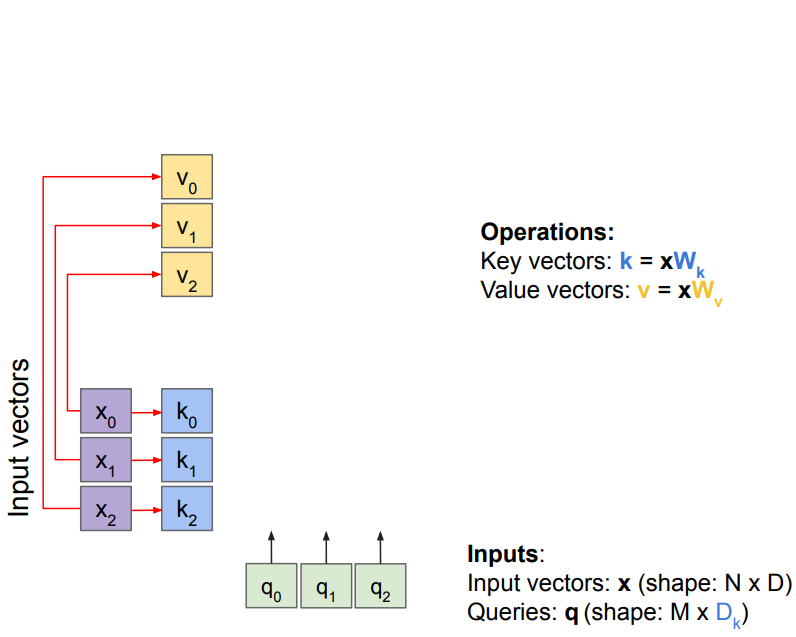
\includegraphics[width=1.0\textwidth,height=1.0\textheight,keepaspectratio]{images/advanced-cv/attention_25.png}
    \end{figure}
    }

    \only<6>{
    \begin{figure}
    \centering
    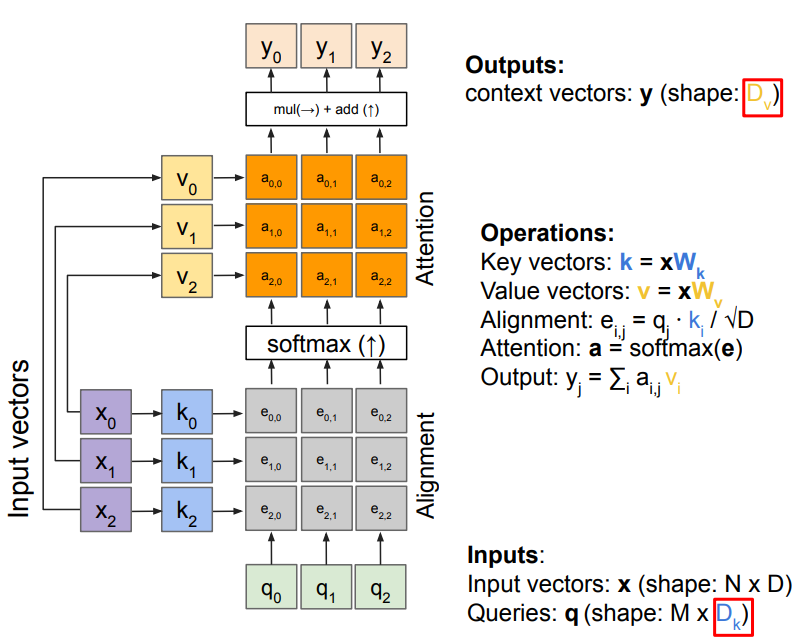
\includegraphics[width=1.0\textwidth,height=1.0\textheight,keepaspectratio]{images/advanced-cv/attention_26.png}
    \end{figure}
    }
        
    \end{column}

    \begin{column}{0.5\textwidth}
    \only<1>{
    \begin{itemize}
        \item The attention operation is permutation invariant.
        \item It does not depend on the ordering of the features.
        \item Stretch $H \times W = N$ into $N$ vectors.
    \end{itemize}
    }

    \only<2>{
    Change $f_{att}(.)$ to a scaled simple dot product:
    \begin{itemize}
        \item Larger dimensions mean more terms in the dot product sum.
        \item Therefore, the variance of the logits is higher. Large-magnitude vectors will produce much higher logits.
        \item As a result, the post-softmax distribution has lower entropy, assuming logits are IID.
        \item Ultimately, these large-magnitude vectors will cause softmax to peak and assign very little weight to all others.
        \item Divide by $\sqrt{D}$ to reduce the effect of large-magnitude vectors.
    \end{itemize}
    }

    \only<3>{
    \begin{itemize}
        \item We can have multiple query vectors.
        \item Each query creates a new output context vector.
    \end{itemize}
    }

    \only<4->{
    \begin{itemize}
        \item Notice that the input vectors are used for both the alignment and the attention calculations.
    \end{itemize}
    }

    \only<5->{
    \begin{itemize}
        \item We can add more expressivity to the layer by adding a different fully connected (FC) layer before each of the two steps.
    \end{itemize}
    }

    \only<6->{
    \begin{itemize}
        \item The input and output dimensions can now change depending on the key and value FC layers.
    \end{itemize}
    }
    
    \end{column}
\end{columns}
\end{frame}
